% FIXME: underscore copyable
% FIXME: %>>% operator

\documentclass{beamer}

\usepackage[orientation=landscape,size=a0,scale=1.4,debug]{beamerposter}
\mode<presentation>{\usetheme{mlr}}

\usepackage[utf8]{inputenc} % UTF-8
\usepackage[english]{babel} % Language
\usepackage{hyperref} % Hyperlinks
\usepackage{ragged2e} % Text position
\usepackage[export]{adjustbox} % Image position
\usepackage[most]{tcolorbox}
\usepackage{listings} % for R code
\lstset{language=R,
    basicstyle=\small\ttfamily,
    stringstyle=\color{DarkGreen},
    otherkeywords={0,1,2,3,4,5,6,7,8,9},
    morekeywords={TRUE,FALSE},
    deletekeywords={data,frame,length,as,character},
    keywordstyle=\color{blue},
    commentstyle=\color{DarkGreen},
}

\title{mlr3pipelines :\,: CHEAT SHEET} % Package title in header, \, adds thin space between ::
\newcommand{\packagedescription}{ % Package description in header
	The \textbf{mlr3pipelines} package is a dataflow programming toolkit for mlr3.
}

\newlength{\columnheight} % Adjust depending on header height
\setlength{\columnheight}{84cm} 

\newtcolorbox{codebox}{%
	sharp corners,
	leftrule=0pt,
	rightrule=0pt,
	toprule=0pt,
	bottomrule=0pt,
	hbox}

\newtcolorbox{codeboxmultiline}[1][]{%
	sharp corners,
	leftrule=0pt,
	rightrule=0pt,
	toprule=0pt,
	bottomrule=0pt,
	#1}

\newtcolorbox{codeboxinline}{%
	sharp corners,
	leftrule=0pt,
	rightrule=0pt,
	toprule=0pt,
	bottomrule=0pt,
	hbox,
	nobeforeafter,
	tcbox raise base}

\newcommand{\codeinline}[1]{\begin{codeboxinline}#1\end{codeboxinline}}

\begin{document}
\begin{frame}[fragile]{}
	\begin{columns}
		\begin{column}{.245\textwidth}
			\begin{beamercolorbox}[center]{postercolumn}
				\begin{minipage}{.98\textwidth}
					\parbox[t][\columnheight]{\textwidth}{
						\begin{myblock}{Intro}
              The mlr3pipelines package is an extension for the \href{https://github.com/mlr-org/mlr3}{mlr3} package and provides so-called \codeinline{PipeOp}s (pipeline operators) which can then be connected with directed edges in a \codeinline{Graph}.
            \end{myblock}
						\begin{myblock}{PipeOps}
              A \codeinline{PipeOp} is an instance of an R6 class and represents transformative operations on input leading to output but behaves differently during a ``training phase'' and ``prediction phase''. While the training phase will typically generate a certain model that is saved as an internal state, the prediction phase will operate on the input data depending on the trained model. \codeinline{PipeOp}s can have multiple inputs and outputs (see \textit{\$input} and \textit{\$output}).
              \\
              \\
              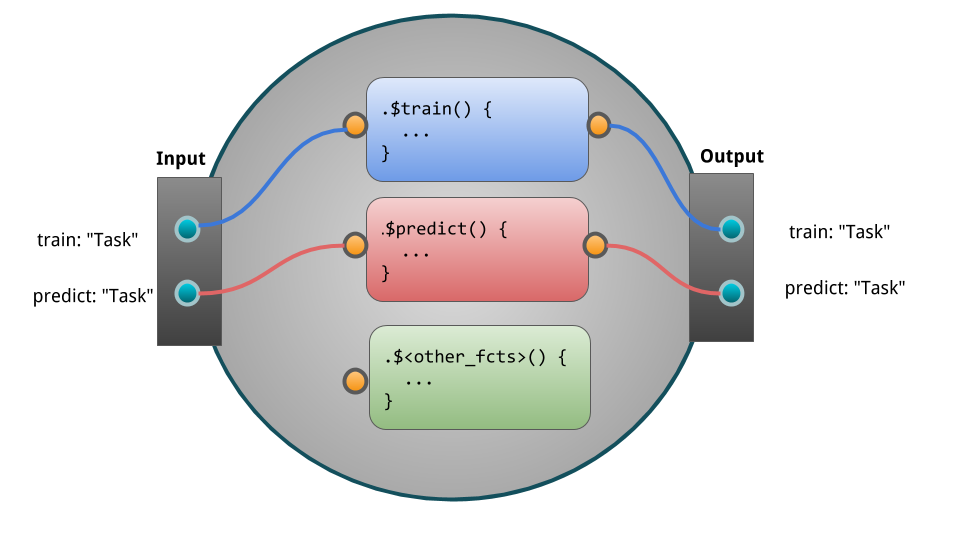
\includegraphics[width=\textwidth]{img/po_viz.png}
              Important methods and slots:
              \begin{itemize}
                \item \textit{\$train()} takes a list of input arguments and turns them into a list of outputs while saving a state in \textit{\$state}
                \item \textit{\$predict()} takes a list of input arguments and turns them into a list of outputs relying on the saved \textit{\$state}
                \item \textit{\$state} contains the ``model'' trained with \textit{\$train()} and utilized during \textit{\$predict()}
              \end{itemize}
              \ \\
              \codeinline{PipeOp}s that are provided by the mlr3package:
              \begin{codebox}
                as.data.table(mlr\_pipeops)
              \end{codebox}
              \ \\
              Construction of a \textit{<key>} \codeinline{PipeOp}:
              \begin{codebox}
                po = mlr\_pipeops\$get("<key>")
              \end{codebox}
						\end{myblock}
						\vfill}
				\end{minipage}
			\end{beamercolorbox}
		\end{column}
		\begin{column}{.245\textwidth}
			\begin{beamercolorbox}[center]{postercolumn}
				\begin{minipage}{.98\textwidth}
					\parbox[t][\columnheight]{\textwidth}{
						\begin{myblock}{Graphs}
              A \codeinline{Graph} is an instance of an R6 class, collecting \codeinline{PipeOp}s with ``edges'' mandating that data should be flowing along them. Edges always pass between \codeinline{PipeOp} \textit{channels}.
              \\
              \\
              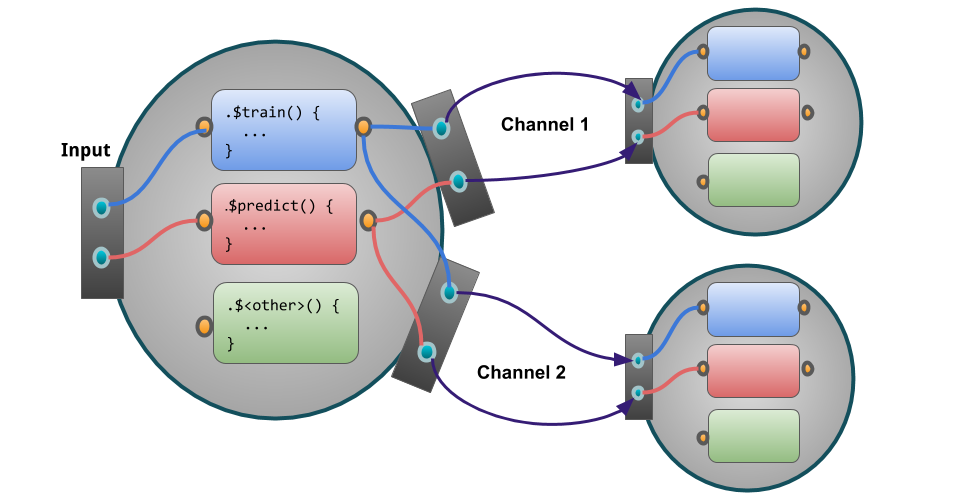
\includegraphics[width=\textwidth]{img/po_multi_viz.png}
              Construction (empty \codeinline{Graph}):
              \begin{codebox}
                gr = Graph\$new()
              \end{codebox}
              \ \\
              Adding \codeinline{PipeOp}s:
              \begin{codeboxmultiline}[width=22cm]
                gr\$add\_pipeop(mlr\_pipeops\$get("<key1>"))\\
                gr\$add\_pipeop(mlr\_pipeops\$get("<key2>"))
              \end{codeboxmultiline}
              \ \\
              Connecting the \codeinline{PipeOp}s:
              \begin{codebox}
                gr\$add\_edge("<key1>", "<key2>")
              \end{codebox}
              \ \\
              Printing and plotting the \codeinline{Graph}:
              \begin{codeboxmultiline}[width=12cm]
                print(gr)\\
                gr\$plot(html = TRUE)
              \end{codeboxmultiline}
              \ \\
              Assessing the \codeinline{PipeOp}s of a \codeinline{Graph}:
              \begin{codebox}
                gr\$pipeops
              \end{codebox}
              \ \\
              A \codeinline{Graph} itself has a \textit{\$train()} and \textit{\$predict()} method that accept data and propagate this data through the network of \codeinline{PipeOp}s. The return value corresponds to the output of the \codeinline{PipeOp} output channels that are not connected to other \codeinline{PipeOp}s.\\
						\end{myblock}
						\vfill}
				\end{minipage}
			\end{beamercolorbox}
		\end{column}
		\begin{column}{.245\textwidth}
			\begin{beamercolorbox}[center]{postercolumn}
				\begin{minipage}{.98\textwidth}
					\parbox[t][\columnheight]{\textwidth}{
            \begin{myblock}{Syntactic Sugar}
              To build a \codeinline{Graph} from layers, use the \codeinline{\%>>\%} operator. It takes either a \codeinline{PipeOp} or a \codeinline{Graph} on each of its sides and connects all of the outputs of its left-hand side to the inputs of its right-hand side:
              \begin{codeboxmultiline}[width=18cm]
                mlr\_pipeops\$get("<key1>") \%>>\%
                \hspace*{1ex}mlr\_pipeops\$get("<key2>")
              \end{codeboxmultiline}
              \ \\
              The \codeinline{gunion()} operator takes \codeinline{PipeOp}s and \codeinline{Graphs} and arranges them next to each other creating a disjoint graph union:
              \begin{codeboxmultiline}[width=20cm]
                gunion(list(mlr\_pipeops\$get("<key1>"),\\
                \hspace*{1ex}mlr\_pipeops\$get("<key2>"))
              \end{codeboxmultiline}
						\end{myblock}
						\begin{myblock}{Learners in Graphs}
              A \codeinline{PipeOpLearner} takes a any mlr3 \codeinline{Learner} and produces a \codeinline{PipeOp}. This \codeinline{PipeOp} can be used after a preprocessing pipeline:
              \begin{codebox}
                mlr\_pipeops\$get("learner", "mlr\_learners\$get("<key>"))
              \end{codebox}
            \end{myblock}
						\begin{myblock}{Graphs in Learners}
              Dual to this procedure, a \codeinline{Graph} can be wrapped in a \codeinline{Learner}, resulting in a \codeinline{GraphLearner}:
              \begin{codebox}
                GraphLearner\$new(gr)
              \end{codebox}
            \end{myblock}
						\vfill}
				\end{minipage}
			\end{beamercolorbox}
		\end{column}
    \begin{column}{.245\textwidth}
			\begin{beamercolorbox}[center]{postercolumn}
				\begin{minipage}{.98\textwidth}
					\parbox[t][\columnheight]{\textwidth}{
            \begin{myblock}{Hyperparameters}
              mlr3pipelines relies on the paradox package to provide parameters that can modify a \codeinline{PipeOp}'s behavior. To inspect the parameters use:
              \begin{codebox}
                mlr\_pipeops\$get("<key>")\$param\_set
              \end{codebox}
              \ \\
              To set or retrieve a parameter, the \codeinline{\$param\_set\$values} slot can be accessed. Alternatively, \codeinline{param\_vals} can be specified during construction:
              \begin{codebox}
                mlr\_pipeops\$get("<key>", param\_vals = list(<values>)
              \end{codebox}
              \ \\
              Note that in a \codeinline{Graph}, the parameters of all \codeinline{PipeOp}'s are collected together.
              Finally, note that both a \codeinline{PipeOpLearner} and \codeinline{GraphLearner} preserve parameters of the objects they encapsulate.
            \end{myblock}
						\vfill}
				\end{minipage}
			\end{beamercolorbox}
		\end{column}
	\end{columns}
\end{frame}
\end{document}
